%!TEX root = main.tex
\section{Moment Averaging \& Post-Selection Estimators}
\label{sec:avg}
In the preceding section we derived the FMSC as an asymptotically unbiased estimator of the AMSE of a candidate estimator.
Besides presenting simulation results, however, we have thus far said nothing about the sampling properties of the FMSC selection procedure itself.
Because it is constructed from $\widehat{\tau}$ the FMSC is a random variable, even in the limit.
Combining Corollary \ref{cor:tautau} with Equation \ref{eq:fmsc} gives the following.
\begin{cor}[Limit Distribution of FMSC]
\label{cor:FMSClimit}
	Under Assumptions \ref{assump:drift}, \ref{assump:highlevel} and \ref{assump:Identification}, $FMSC_n(S) \rightarrow_d FMSC_S(\tau, M)$, where
	\begin{eqnarray*}
		\mbox{FMSC}_S(\tau,M) &=& \nabla_\theta\mu(\theta_0)'K_S\Xi_S \left\{\left[\begin{array}{cc}0&0\\0& B(\tau,M) \end{array}\right] + \Omega\right\}\Xi_S'K_S'\nabla_\theta\mu(\theta_0)\\
		B(\tau,M) &=& (\Psi M + \tau)(\Psi M + \tau)' - \Psi \Omega \Psi.
	\end{eqnarray*}
\end{cor}


Because the FMSC is itself random, so is the FMSC-selected estimator.
This means that the FMSC is a ``conservative'' rather than ``consistent'' selection procedure.
While this lack of consistency may sound like a ``bug'' it is in fact a desirable feature of the FMSC for two reasons.
First, as discussed above, the goal of the FMSC is not to consistently select the correct moment conditions: it is to choose an estimator with a low finite-sample MSE as approximated by AMSE.
In fact, the goal of consistent selection is very much at odds with that of controlling estimator risk.
As explained by \cite{Yang2005} and \cite{LeebPoetscher2008}, the worst-case risk of a consistent selection procedure \emph{diverges} with sample size. 

Second, while we know from simulation studies that selection can dramatically change the sampling distribution of our estimators, the asymptotics of consistent selection give the misleading impression that this effect can be ignored.
For example Lemma 1.1 of \citet[p.\ 168]{Poetscher1991}, which states that the limit distributions of an estimator pre- and post-consistent selection are identical, has been interpreted by some as evidence that consistent selection is innocuous. 
\citet[pp.\ 179--180]{Poetscher1991} makes it very clear, however, this result does not hold uniformly in the parameter space and hence ``only creates an illusion of conducting valid inference'' \citep[p.\ 22]{LeebPoetscher2005}.
Figure \ref{fig:consist} illustrates this problem using the simulation experiment from Section \ref{sec:fmscsim} with a sample size of $500$ and $\gamma = 0.4$, $\rho= 0.2$.
At these parameter values, $w$ is an invalid instrument.
Because they are consistent criteria, and hence will exclude any invalid instruments in the limit, a na\"{i}ve reading of P\"{o}tscher's Lemma 1.1 would suggest that the post-selection distributions of GMM-BIC and HQ should be close to that of the valid estimator, given in dashed lines.
This is emphatically not the case: both post-selection distributions are highly non-normal mixtures. 
\begin{figure}[htbp]
\begin{center}
	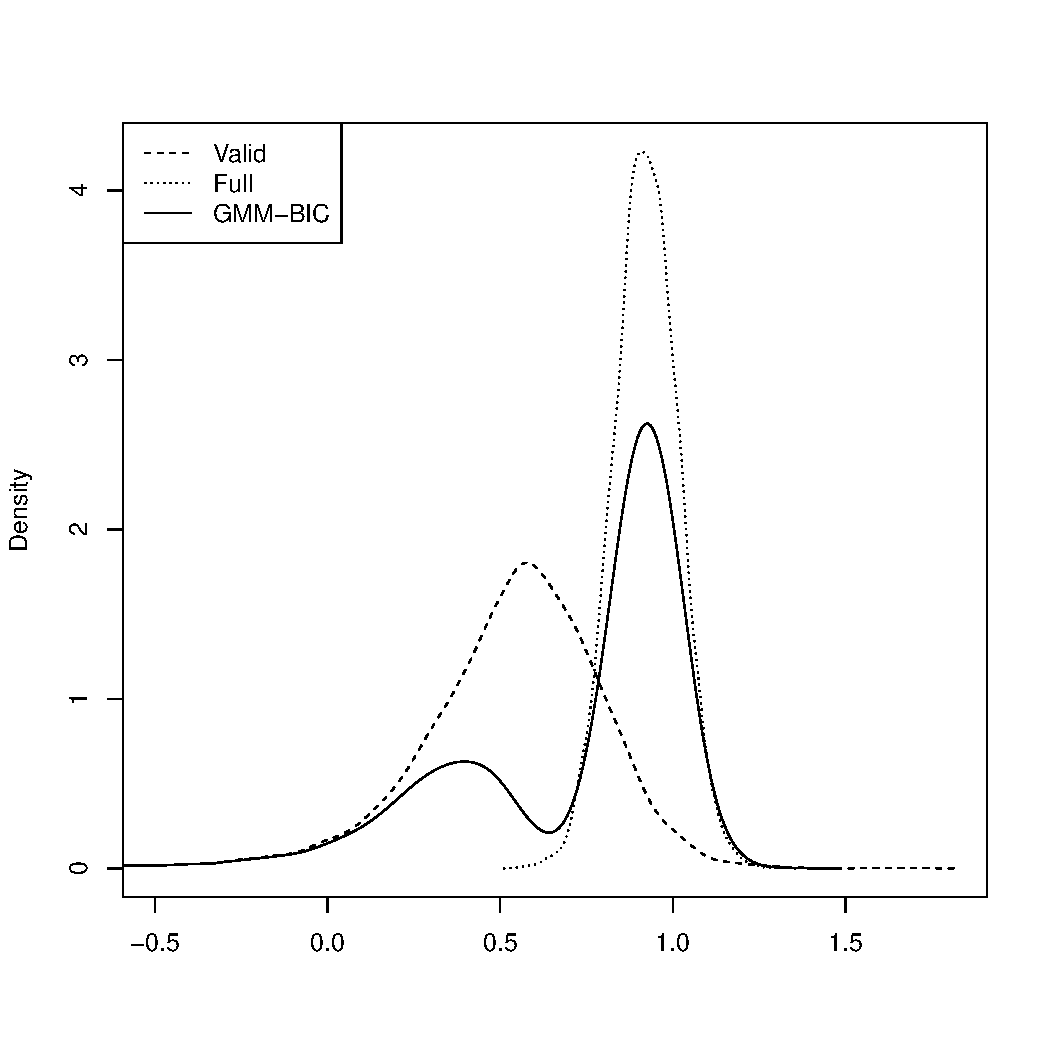
\includegraphics[scale = 0.48]{GMM_BIC}
	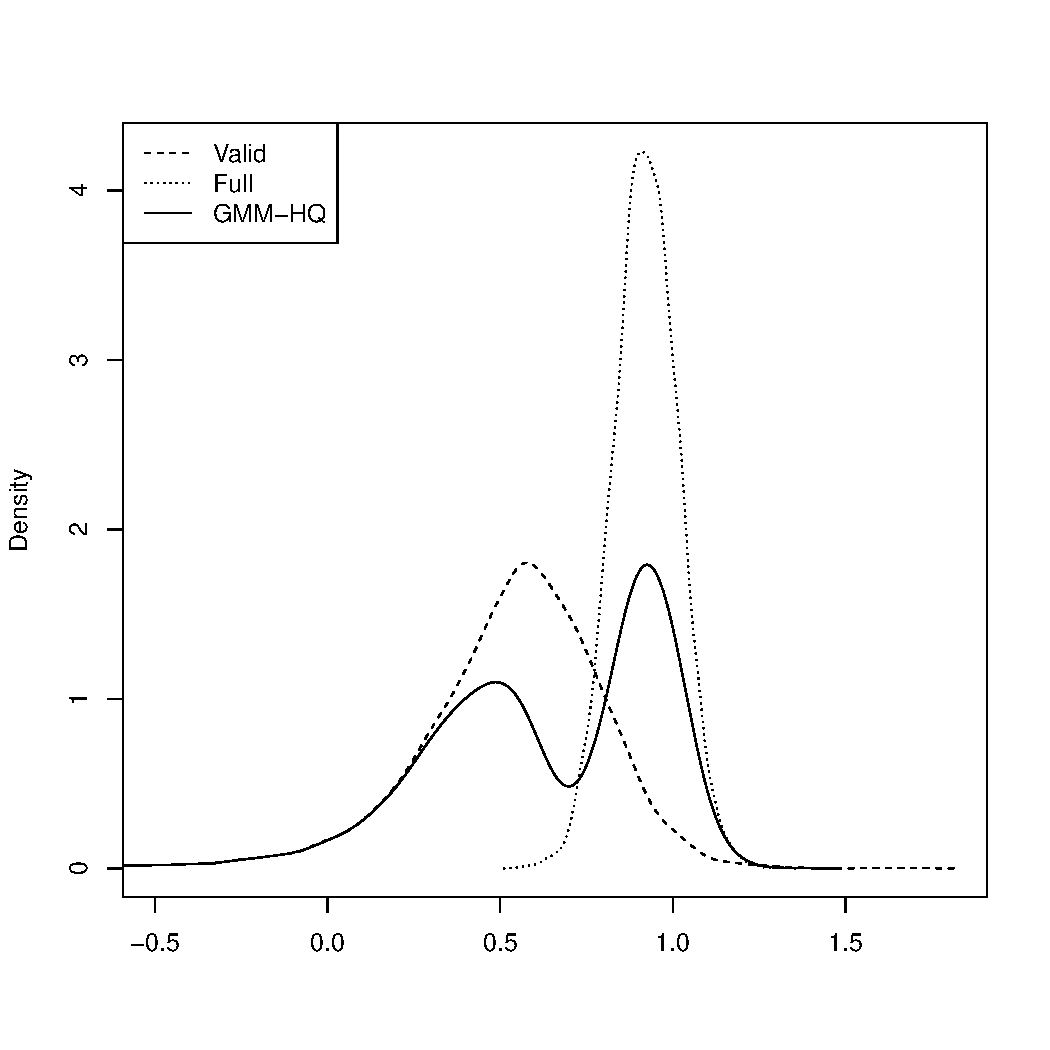
\includegraphics[scale = 0.48]{GMM_HQ}
\caption{ \small Post-selection distributions for the estimated effect of $x$ on $y$ in Equation \ref{eq:secondstage} with $\gamma = 0.4$, $\rho = 0.2$, $N=500$. The distribution post-GMM-BIC selection appears in the top panel, while the distribution post-GMM-HQ selection appears in the bottom panel. The distribution of the full estimator is given in dotted lines while that of the valid estimator is given in dashed lines in each panel. All distributions are calculated by kernel density estimation based on 10,000 simulation replications generated from Equations \ref{eq:secondstage}--\ref{eq:varmatrix}.}
\label{fig:consist}
\end{center}
\end{figure}
While Figure \ref{fig:consist} examines only one point in the parameter space the problem is more general, as shown by Table \ref{tab:BICcov}. 
The empirical coverage probabilities of traditional $95\%$ confidence intervals are far lower than their nominal level over the majority of the parameter space and the lack of uniformity is striking: small changes in parameters lead to large changes in coverage.

% latex.default(cover.BIC, file = outfilename, greek = TRUE, numeric.dollar = FALSE,      na.blank = TRUE, landscape = FALSE, rowname = NULL, append = TRUE) 
%
\begin{table}[!tbp]
\caption{Coverage post-GMM-BIC moment selection (nominal 95\%).}
\label{tab:BICcov}
\small
 \begin{center}
 \begin{tabular}{r|rrrrrrrrr}\hline\hline
&\multicolumn{9}{c}{$\rho = Cov(w,u)$}\\
\multicolumn{1}{c|}{$N = 500$}&\multicolumn{1}{c}{0}&\multicolumn{1}{c}{0.05}&\multicolumn{1}{c}{0.10}&\multicolumn{1}{c}{0.15}&\multicolumn{1}{c}{0.20}&\multicolumn{1}{c}{0.25}&\multicolumn{1}{c}{0.30}&\multicolumn{1}{c}{0.35}&\multicolumn{1}{c}{0.40}\tabularnewline
\hline
0.0&0.92&0.92&0.92&0.93&0.92&0.92&0.92&0.92&0.93\tabularnewline
0.1&0.92&0.83&0.77&0.83&0.90&0.92&0.93&0.92&0.92\tabularnewline
0.2&0.93&0.76&0.55&0.57&0.74&0.86&0.89&0.90&0.91\tabularnewline
0.3&0.93&0.75&0.45&0.35&0.50&0.69&0.80&0.85&0.88\tabularnewline
0.4&0.93&0.75&0.40&0.22&0.31&0.48&0.63&0.74&0.80\tabularnewline
0.5&0.93&0.75&0.38&0.18&0.20&0.32&0.46&0.59&0.68\tabularnewline
0.6&0.94&0.76&0.38&0.14&0.14&0.23&0.32&0.43&0.53\tabularnewline
\multirow{4}{5mm}{\begin{sideways}\parbox{1mm}{$\gamma\;$=$\;Cov(w,x)$}\end{sideways}}
0.7&0.94&0.76&0.37&0.12&0.11&0.16&0.24&0.32&0.42\tabularnewline
0.8&0.93&0.76&0.37&0.11&0.08&0.12&0.18&0.25&0.33\tabularnewline
0.9&0.94&0.75&0.37&0.11&0.07&0.10&0.14&0.19&0.25\tabularnewline
1.0&0.93&0.76&0.37&0.10&0.06&0.08&0.11&0.16&0.20\tabularnewline
1.1&0.93&0.77&0.37&0.10&0.06&0.07&0.10&0.13&0.16\tabularnewline
1.2&0.94&0.77&0.38&0.10&0.05&0.06&0.08&0.11&0.14\tabularnewline
1.3&0.94&0.77&0.38&0.10&0.04&0.05&0.07&0.09&0.12\tabularnewline
\hline
\end{tabular}
\end{center}
\footnotesize
\begin{tablenotes}
\item Values are calculated by simulating from Equations \ref{eq:secondstage}--\ref{eq:varmatrix} with $10,000$ replications.
\end{tablenotes}
\end{table}

In constrast to those of consistent selection, the asymptotics of \emph{conservative} selection  under local mis-specification provide a far more accurate picture of the distribution of post-selection estimators.
The point is \emph{not} that conservative criteria -- such as the FMSC, GMM-AIC and $J$-test at a fixed significance level -- are immune to the effects of selection on inference.
%The coverage probabilities for post-FMSC estimators given in Table \ref{tab:FMSCconf}, for example, show that this is not the case.
Rather, it is that conservative criteria can be studied in a framework that allows us to capture the non-normality that is so apparent from Figure \ref{fig:consist} in our limit theory.  
To this end, the present section derives the asymptotic distribution of generic ``moment average'' estimators by extending the idea behind the frequentist model average estimators of \cite{HjortClaeskens}. 
Such estimators are interesting in their own right and include, as a special case, a variety of post-conservative moment selection estimators including the FMSC.
Although their limit distributions are complicated, it remains possible to construct asymptotically valid confidence intervals for moment average estimators using a two-step, simulation-based procedure.
We begin by defining moment average estimators in general and considering some examples before presenting the procedure for constructing valid confidence intervals.

\subsection{Moment Average Estimators}
A generic moment average estimator takes the form
\begin{equation}
	\label{eq:avg}
	\widehat{\mu}=\sum_{S \in \mathscr{S}} \widehat{\omega}_S\widehat{\mu}_S
\end{equation}
where $\widehat{\mu}_S = \mu(\widehat{\theta}_S)$ is the estimator of the target parameter $\mu$ under moment set $S$, $\mathscr{S}$ is the collection of all moment sets under consideration, and $\widehat{\omega}_S$ is shorthand for the value of a data-dependent weight function  $\widehat{\omega}_S=\omega(\cdot, \cdot)$ evaluated at moment set $S$ and the sample observations $Z_{n1}, \hdots, Z_{nn}$.  
As above $\mu(\cdot)$ is a $\mathbb{R}$-valued, $Z$-almost surely continuous function of $\theta$ that is differentiable in an open neighborhood of $\theta_0$. When $\widehat{\omega}_S$ is an indicator, taking on the value one at the moment set moment set that minimizes some moment selection criterion, $\widehat{\mu}$ is a post-moment selection estimator. To characterize the limit distribution of $\widehat{\mu}$, we impose the following conditions on $\widehat{\omega}_S$.
\begin{assump}[Conditions on the Weights]\mbox{}
\label{assump:weights}
\begin{enumerate}[(a)]
	\item $\sum_{S \in \mathscr{S}} \widehat{\omega}_S = 1$, almost surely 
	\item For each $S\in \mathscr{S}$, $\widehat{\omega}_S \rightarrow_d\varphi_S(\tau, M)$, an almost-surely continuous function of $\tau$, $M$ and consistently estimable constants only.
\end{enumerate}
\end{assump}

\begin{cor}[Asymptotic Distribution of Moment-Average Estimators]
\label{cor:momentavg}
Under Assumption \ref{assump:weights} and the conditions of Theorem \ref{thm:normality},
	$$\sqrt{n}\left(\widehat{\mu} -  \mu_0\right) \rightarrow_{d}\Lambda(\tau) =  -\nabla_\theta\mu(\theta_0)'\left[\sum_{S \in \mathscr{S}} \varphi_S(\tau,M) K_S\Xi_S\right] \left(M + \left[\begin{array}
	{c} 0 \\ \tau
\end{array} \right]\right).$$
\end{cor}
Notice that the limit random variable from Corollary \ref{cor:momentavg}, denoted $\Lambda(\tau)$, is a \emph{randomly weighted average} of the multivariate normal vector $M$. 
Hence, $\Lambda(\tau)$ is non-normal. 
This is precisely the behavior that Figure \ref{fig:consist} suggests our limit theory should capture.
The conditions of Assumption \ref{assump:weights} are fairly mild. 
Requiring that the weights sum to one ensures that $\widehat{\mu}$ is a consistent estimator of $\mu_0$ and leads to a simpler expression for the limit distribution. 
While somewhat less transparent, the second condition is satisfied by weighting schemes based on a number of familiar moment selection criteria.
We see immediately from Corollary \ref{cor:FMSClimit}, for example, that the FMSC converges in distribution to a function of $\tau$, $M$ and consistently estimable constants only. 
The same ss true for the $J$-test statistic, as we see from the following result. 
\begin{thm}[Distribution of $J$-Statistic under Local Mis-Specification] 
\label{pro:jstat}
	Define the J-test statistic as per usual by $J_n(S)  = n \left[\Xi_S f_n(\widehat{\theta}_S)\right]' \widehat{\Omega}^{-1}\left[\Xi_S f_n(\widehat{\theta}_S)\right]$ where $\widehat{\Omega}^{-1}_S$ is a consistent estimator of $\Omega_S^{-1}$. Then, under the conditions of Theorem \ref{thm:normality}, we have $J_n(S) \rightarrow_dJ_S(\tau, M)$ where
		$$J_S(\tau, M)=[\Omega_S^{-1/2}(M_S + \tau_S)]' (I - P_S)[\Omega_S^{-1/2}\Xi_S(M_S + \tau_S)],$$
$M_S = \Xi_S M$, $\tau_S' = (0', \tau')\Xi_S'$, and $P_S$ is the projection matrix formed from the GMM identifying restrictions $\Omega^{-1/2}_S F_S$.
\end{thm}
Hence, normalized weights constructed from almost-surely continuous functions of either the FMSC or the $J$-test statistic satisfy Assumption \ref{assump:weights}. 

Post-selection estimators are merely a special cases of moment average estimators.
To see why, consider the weight function
$$\widehat{\omega}_S^{MSC} = \mathbf{1}\left\{\mbox{MSC}_n(S) = \min_{S'\in \mathscr{S}} \mbox{MSC}_n(S')\right\}$$where $\mbox{MSC}_n(S)$ is the value of some moment selection criterion evaluated at the sample observations $Z_{n1}\hdots, Z_{nn}$. 
Now suppose $\mbox{MSC}_n(S) \rightarrow_d\mbox{MSC}_S(\tau,M)$, a function of $\tau$, $M$ and consistently estimable constants only. 
Then, so long as the probability of ties, $P\left\{\mbox{MSC}_S(\tau,M) = \mbox{MSC}_{S'}(\tau,M) \right\}$, is zero for all $S\neq S'$, the continuous mapping theorem gives 
	$$\widehat{\omega}_S^{MSC} \rightarrow_d \mathbf{1}\left\{\mbox{MSC}_S(\tau,M) = \min_{S'\in \mathscr{S}} \mbox{MSC}_{S'}(\tau,M)\right\}$$ 
satisfying Assumption \ref{assump:weights} (b). 
Thus, post-selection estimators based on the FMSC, the downward $J$-test procedure, GMM-BIC, GMM-HQ, and GMM-AIC all fall within the ambit of \ref{cor:momentavg}. 
GMM-BIC and GMM-HQ, however, are not particularly interesting under local mis-specification.
Intuitively, because they aim to select all valid moment conditions w.p.a.1, we would expect that under Assumption \ref{assump:drift} they simply choose the full moment set in the limit. 
The following result states that this intuition is correct. 
\begin{thm}[Consistent Criteria under Local Mis-Specification]
\label{pro:andrews}
Consider a moment selection criterion of the form $MSC(S) = J_n(S) - h(|S|)\kappa_n$, where $h$ is strictly increasing,  $\lim_{n\rightarrow \infty}\kappa_n = \infty$, and $\kappa_n = o(n)$. Under the conditions of Theorem \ref{thm:normality}, $MSC(S)$ selects the full moment set with probability approaching one.
\end{thm}
The preceding result is a special case of a more general phenomenon: consistent selection procedures cannot detect model violations of order $O(n^{-1/2})$.
Because moment selection using the GMM-BIC or HQ leads to weights with a degenerate asymptotic distribution, one that does not capture the effects of selection on inference, these criteria are not considered further below.